\documentclass[tikz,border=0pt,11pt]{standalone}
\usepackage[T1]{fontenc}
\usepackage[utf8]{inputenc}
\usepackage{lmodern,amsmath,amssymb}
\usepackage[swedish]{babel}
\usetikzlibrary{arrows.meta,calc,positioning,decorations.pathmorphing,decorations.pathreplacing,patterns,shadings}
\definecolor{navy}{HTML}{102F40}
\definecolor{teal}{HTML}{147D78}
\definecolor{lightteal}{HTML}{E6F1ED}
\definecolor{gold}{HTML}{B88B3B}
\definecolor{palegold}{HTML}{F7EEDB}
\definecolor{rust}{HTML}{B6533B}
\definecolor{palerust}{HTML}{FAEAE4}
\definecolor{paper}{HTML}{F7F5EE}
\definecolor{muted}{HTML}{5B6D72}
\definecolor{line}{HTML}{D6DED8}
\renewcommand{\familydefault}{\sfdefault}
\newcommand{\atom}[5]{\shade[ball color=#3!70] (#1,#2) circle (#5);\node[text=white,font=\bfseries\small] at (#1,#2){#4};}
\newcommand{\water}[3]{\begin{scope}[shift={(#1,#2)},scale=#3]\draw[navy!45,line width=2pt] (-.3,.22)--(0,0)--(.3,.22);\atom{0}{0}{rust}{O}{.22}\atom{-.3}{.22}{teal}{H}{.15}\atom{.3}{.22}{teal}{H}{.15}\end{scope}}
\newcommand{\panel}[4]{\filldraw[fill=white,draw=line,rounded corners=5pt] (#1,#2) rectangle ++(#3,#4);}
\newcommand{\note}[4]{\node[txt,text width=#3cm] at (#1,#2){#4};}
\tikzset{txt/.style={anchor=north west,align=left,text=navy,font=\small},
 head/.style={anchor=west,text=navy,font=\bfseries\large},
 label/.style={align=center,text=navy,font=\small},
 smalllabel/.style={align=center,text=muted,font=\footnotesize},
 arrow/.style={-{Latex[length=2.5mm,width=1.8mm]},line width=1.2pt,draw=teal},
 goldarrow/.style={-{Latex[length=2.5mm]},line width=1.2pt,draw=gold},
 rustarrow/.style={-{Latex[length=2.5mm]},line width=1.2pt,draw=rust},
 dashedarrow/.style={arrow,dashed},
 badge/.style={fill=lightteal,rounded corners=3pt,text=teal,font=\bfseries\small,inner sep=5pt}}
\begin{document}
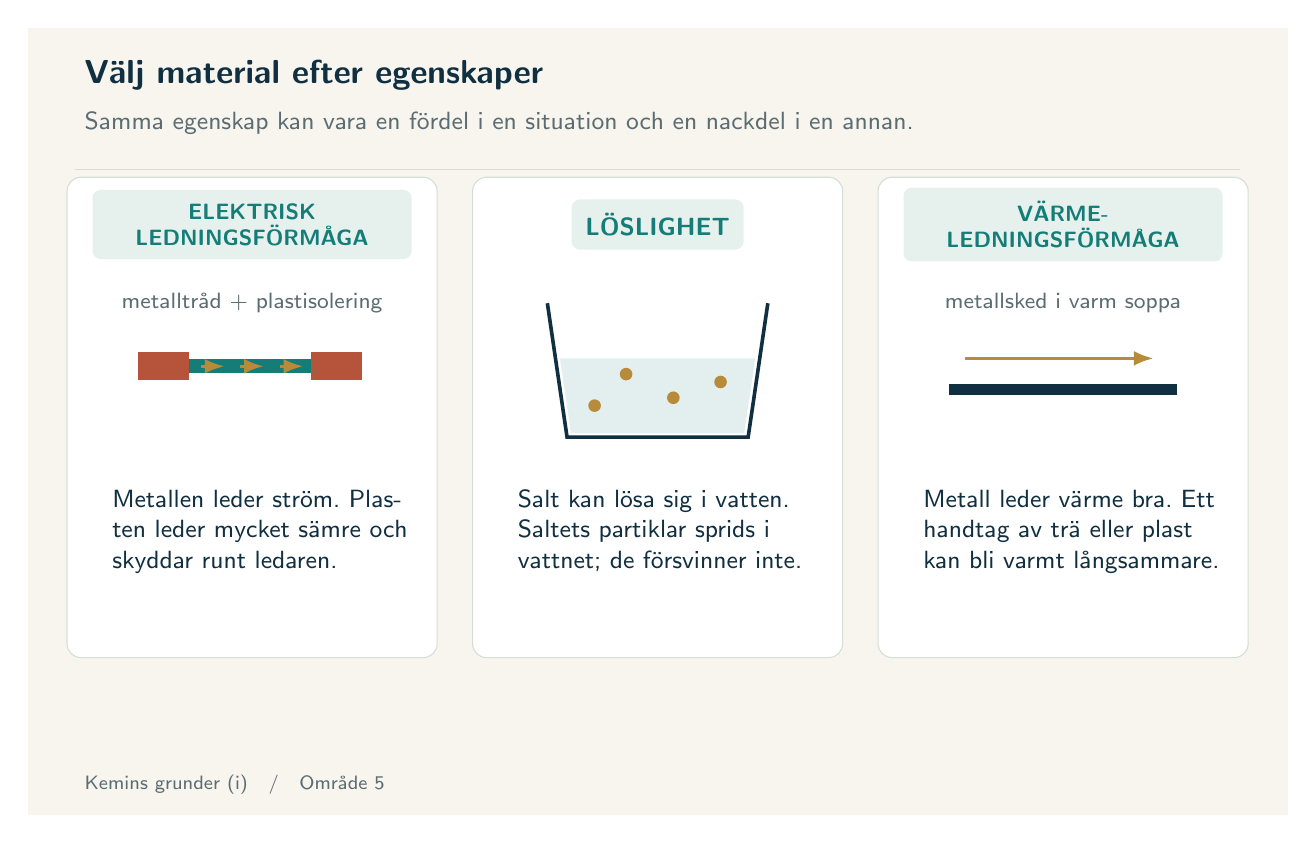
\begin{tikzpicture}[x=1cm,y=1cm]
\path[use as bounding box] (0,0) rectangle (16,10);
\fill[paper] (0,0) rectangle (16,10);
\node[head] at (.6,9.4){Välj material efter egenskaper};
\note{.6}{9.05}{14.8}{\textcolor{muted}{Samma egenskap kan vara en fördel i en situation och en nackdel i en annan.}}
\draw[line] (.6,8.2)--(15.4,8.2);

\foreach \x in {.5,5.65,10.8}{\panel{\x}{2}{4.7}{6.1}}
\node[badge,align=center,text width=3.7cm,font=\bfseries\footnotesize] at (2.85,7.5){ELEKTRISK\\ LEDNINGSFÖRMÅGA};\node[badge] at (8,7.5){LÖSLIGHET};\node[badge,align=center,text width=3.7cm,font=\bfseries\footnotesize] at (13.15,7.5){VÄRME-\\ LEDNINGSFÖRMÅGA};
\draw[teal,line width=5pt] (1.4,5.7)--(4.25,5.7);\draw[rust,line width=10pt] (1.4,5.7)--(2.05,5.7);\draw[rust,line width=10pt] (3.6,5.7)--(4.25,5.7);\foreach \x in {2.2,2.7,3.2}{\draw[goldarrow] (\x,5.7)--++(.3,0);}
\node[smalllabel,text width=3.5cm] at (2.85,6.5){metalltråd + plastisolering};
\draw[navy,line width=1.3pt] (6.6,6.5)--(6.85,4.8)--(9.15,4.8)--(9.4,6.5);\fill[teal!12] (6.76,5.8)--(9.24,5.8)--(9.1,4.85)--(6.9,4.85)--cycle;\foreach \x/\y in {7.2/5.2,7.6/5.6,8.2/5.3,8.8/5.5}{\fill[gold] (\x,\y) circle(.08);}
\draw[navy,line width=4pt] (11.7,5.4)--(14.6,5.4);\draw[goldarrow] (11.9,5.8)--(14.3,5.8);\node[smalllabel] at (13.15,6.5){metallsked i varm soppa};
\note{.95}{4.25}{3.8}{Metallen leder ström. Plasten leder mycket sämre och skyddar runt ledaren.}
\note{6.1}{4.25}{3.8}{Salt kan lösa sig i vatten. Saltets partiklar sprids i vattnet; de försvinner inte.}
\note{11.25}{4.25}{3.8}{Metall leder värme bra. Ett handtag av trä eller plast kan bli varmt långsammare.}\node[anchor=west,text=muted,font=\scriptsize] at (.6,.38){Kemins grunder (i)\quad /\quad Område 5};

\end{tikzpicture}\end{document}
